\documentclass{article}
\usepackage[preprint]{neurips_2025}
\setcitestyle{numbers,square}

\usepackage[utf8]{inputenc} % allow utf-8 input
\usepackage[T1]{fontenc}    % use 8-bit T1 fonts
\usepackage{hyperref}       % hyperlinks
\usepackage{url}            % simple URL typesetting
\usepackage{booktabs}       % professional-quality tables
\usepackage{amsfonts}       % blackboard math symbols
\usepackage{nicefrac}       % compact symbols for 1/2, etc.
\usepackage{microtype}      % microtypography
\usepackage{xcolor}         % colors
\usepackage{amsmath}
\usepackage{algorithm,algorithmicx,algpseudocode}
\usepackage{multirow}
\usepackage{graphicx}
\usepackage[colorinlistoftodos,textsize=small]{todonotes}
\usepackage{subcaption}
\captionsetup[table]{skip=10pt}

\DeclareMathOperator*{\argmax}{arg\,max}
\DeclareMathOperator*{\argmin}{arg\,min}


\title{Title}
\author{
  Anonymous Author
  % Theo Farrell \\
  % Department of Computer Science \\
  % Durham University \\
  % \texttt{theodore.farrell@durham.ac.uk} \\
}




\begin{document}

\maketitle

\begin{abstract}
    asdfasdf
\end{abstract}


\section{Introduction}

% ============================================================
% No explicit word limit, but keep it short — the marks are in
% sections 1 and 2. 1-2 paragraphs is plenty.
% Excluded from word count: bibliography, equations, figures.
% ============================================================

% SUGGESTED CONTENT:
%
%   Para 1 — Context and motivation (~3 sentences)
%     Describe the domain gap between game and movie footage.
%     Explain why human regions are the focus (foreground style matters
%     most; background mixing hurts quality in full-frame translation).
%     One sentence on the broader application (game realism enhancement).
%
%   Para 2 — Approach summary (~3 sentences)
%     "We present a pipeline that: (1) extracts human patches via
%      YOLOv8~\cite{jocher2023} with quality-aware selection; (2)
%      classifies patches into five pose categories using a GCN trained
%      on COCO keypoints; (3) selects diverse representative patches via
%      DINOv2 clustering; and (4) applies CUT~\cite{park2020}
%      patch-level style transfer with EMA temporal blending."
%     Reference Figure showing the overall pipeline if you make one.
%
% KEY REFERENCES TO CITE:
%   - CUT: Park et al. (2020), "Contrastive Unpaired Translation" — the core model
%   - CycleGAN: Zhu et al. (2017) — precursor, good for context
%   - YOLOv8: Jocher et al. (2023), ultralytics/ultralytics
%   - DINOv2: Oquab et al. (2023) — for 1.3 embedding
%   - GCN: Kipf & Welling (2017), "Semi-Supervised Classification with GCNs"
%   - ST-GCN (if you implement temporal GCN): Yan et al. (2018)
%
% OPTIONAL FIGURE (no word cost):
%   A pipeline diagram showing the flow 1.1→1.2→1.3→2.1→2.2.
%   Save to: paper/figs/pipeline_overview.pdf


\section{Human Feature Analysis}\label{s:hfa}

% ============================================================
% WORD LIMITS: 1.1 = 100w, 1.2 = 100w, 1.3 = 100w
% EXCLUDED from count: equations, tables, figures, bibliography
% Examiners stop reading at the limit — cut ruthlessly.
% ============================================================

% ============================================================
\subsection{Human Patch Extraction}
% ============================================================
% TASK: adapt DL detection, propose lightweight useful-frame selection,
%       submit 50 patch samples. Evaluate. 100 words.
%
% SUGGESTED STRUCTURE (≈100 words — every word counts):
%   Sentence 1-2: method name, input, output.
%     "We apply YOLOv8m [CITE] to each training video, extracting
%      bounding-box crops of class `person' at every eligible frame."
%   Sentence 3-4: frame selection (the lightweight algorithm):
%     "To avoid redundant frames, we skip frames with inter-frame
%      mean absolute difference below \(\tau_{sc}=8\) (static shots)
%      and enforce a minimum spacing of 10 frames between YOLO calls.
%      Candidate patches are scored by a weighted combination of
%      detection confidence, relative bounding-box area (peak at 15\%
%      of frame), and Laplacian sharpness; greedy diversity sampling
%      then enforces a 10-frame temporal gap per video source."
%   Sentence 5: result.
%     "This yields 4,000 patches from 4 videos (2,000 game, 2,000 movie)."
%
% KEY THINGS TO JUSTIFY:
%   - Why YOLOv8? (SOTA, fast, pretrained on COCO persons)
%   - Why scene-change threshold? (avoids near-static shots)
%   - Why blur threshold differs? (film grain vs game rendering)
%   - Why greedy diversity? (prevents shot-repetition overfitting)
%   - State the extraction thresholds as concrete numbers
%
% EVALUATION (fits in ≤20 words + a figure):
%   - Quote the blur score range from _summary.txt: min 0.6, max 5351.5
%   - Quote how many raw detections → selected (10674 → 4000)
%
% FIGURES:
%   Fig 1a — 5×10 grid of sampled patches (50 required).
%             Sample script: randomly pick 50 from output/extracted_humans/20260314-195748/
%             Save to: paper/figs/patches_sample.pdf (or .png)
%             Caption: "Random sample of 50 extracted human patches."
%
%   Fig 1b (optional, fits in same figure with subcaption) —
%             Histogram of detection scores (before/after selection).
%             Source: output/extracted_humans/20260314-195748/_summary.txt
%             Save to: paper/figs/score_hist.pdf
%             Caption: "Score distribution of raw detections (grey) vs selected (blue)."
%             This gives you empirical justification for the scoring in ≤1 sentence.
%
% LATEX SKELETON:
% \begin{figure}[t]
%   \centering
%   \includegraphics[width=\linewidth]{figs/patches_sample.pdf}
%   \caption{Random sample of 50 extracted human patches from game (top two rows) and movie (bottom three rows) domains.}
%   \label{fig:patches}
% \end{figure}


\subsection{Classification}
% ============================================================
% TASK: classify 1.1 patches into 5 classes, submit 20/class.
%       Explain, justify, evaluate. 100 words.
%
% SUGGESTED STRUCTURE:
%   Sentence 1: define the 5 classes briefly.
%     "We define full-body as both hip keypoints visible with torso,
%      head-and-shoulder as upper body only, front/back by nose
%      visibility, and others for partial/occluded/non-human crops."
%   Sentence 2-3: method.
%     "We detect 17-point COCO keypoints with YOLOv8-pose [CITE],
%      then train a 3-layer Graph Convolutional Network (GCN)~\cite{kipf2017}
%      on the COCO skeleton graph with node features (x, y, confidence).
%      Confidence-weighted global pooling aggregates per-node embeddings
%      to a graph-level vector for 5-class classification."
%   Sentence 4: labels.
%     "Training labels are obtained from manual annotation of \(\sim\)600
%      patches using a custom Flask tool seeded with rule-based keypoint
%      heuristics."
%   Sentence 5: augmentation.
%     "Horizontal flip augmentation (swapping symmetric keypoint pairs)
%      doubles the training set without requiring additional annotations."
%   Sentence 6-7: result (refer to table/figure).
%     "Val accuracy: full-body-back 94.7\%, full-body-front 72.2\%,
%      head-shoulder-back 70.4\%, head-shoulder-front 65.3\%;
%      `others' accuracy is low (9.8\%), discussed below."
%
% KEY THINGS TO JUSTIFY:
%   - Why GCN over MLP/SVM? Pose is a graph structure — edges encode
%     skeletal connectivity; a GCN naturally propagates joint context.
%   - Why confidence-weighted pooling? Low-confidence keypoints
%     (occluded joints) should contribute less to the graph embedding.
%   - Why manual annotations? Rule-based heuristics misclassify
%     ambiguous poses; a brief ablation (training curves plot) shows
%     manual > rule.
%   - `others' failure: acknowledge it — this class is open-set
%     (no consistent pose signature), so low recall is expected.
%     Mitigation in 2.2: hard threshold on keypoint count.
%
% FIGURES:
%   Fig 2a — 4×5 grid of 20 patches per class (4 main classes × 5 each, or
%             20 per class across multiple figures).
%             Sample: randomly pick 20 from each subdir in
%             output/gcn_results/20260320-162455/<class>/
%             Save to: paper/figs/cls_samples_<class>.pdf
%             Tip: one combined figure with subcaptions per class saves space.
%
%   Fig 2b — GCN training curves (loss + accuracy over epochs).
%             Source: output/gcn_results/20260320-162455/training_curves.png
%             Copy to: paper/figs/gcn_training_curves.png
%             Caption: "GCN training and validation curves."
%
%   Table 1 — Per-class val accuracy (already in _summary.txt).
%             Present as a small table. Excluded from word count.
%             Columns: Class | Correct | Total | Accuracy (%)
%
% LATEX SKELETON:
% \begin{table}[t]
%   \centering
%   \caption{GCN per-class validation accuracy.}
%   \label{tab:gcn}
%   \begin{tabular}{lrrr}
%     \toprule
%     Class & Correct & Total & Acc.\ (\%) \\
%     \midrule
%     Full-body front    & 52 & 72  & 72.2 \\
%     Full-body back     & 18 & 19  & 94.7 \\
%     Head-shoulder front& 49 & 75  & 65.3 \\
%     Head-shoulder back & 19 & 27  & 70.4 \\
%     Others             &  5 & 51  &  9.8 \\
%     \bottomrule
%   \end{tabular}
% \end{table}


\subsection{Training Data Selection}
% ============================================================
% TASK: select most useful patches for style-transfer training.
%       Own observations/insights required. Submit 50 samples. 100 words.
%
% SUGGESTED STRUCTURE:
%   Sentence 1: observation / motivation.
%     "Inspection of extracted patches reveals substantial visual
%      redundancy: consecutive frames of the same shot produce
%      near-identical crops. Training CUT~\cite{park2020} on such
%      data risks overfitting the generator to specific shot compositions
%      rather than learning a domain-level style."
%   Sentence 2-3: method.
%     "We embed all non-`others' patches with DINOv2 ViT-B/14~\cite{oquab2023}
%      and apply K-Means independently within each class\,\(\times\)\,domain
%      group, allocating \(k \propto\) group size from a total budget of
%      2,000 patches.  The patch nearest (cosine distance) to each centroid
%      is selected as the most representative example."
%   Sentence 4: domain balance rationale.
%     "Processing game and movie groups independently preserves
%      the domain balance required by CUT's unpaired discriminator."
%   Sentence 5: result/figure reference.
%     "The resulting selection spans all pose classes and both domains;
%      Figure~\ref{fig:umap} confirms that DINOv2 clusters reflect
%      meaningful pose and domain variation."
%
% KEY THINGS TO JUSTIFY:
%   - Why DINOv2? Pretrained vision transformer captures high-level
%     semantic similarity better than pixel-level hashing or VGG features.
%     Cite: Oquab et al. (2023) DINOv2.
%   - Why per-(class × domain) independently? Maintains class and domain
%     balance for CUT; prevents majority-class clusters from absorbing
%     minority-class patches.
%   - Why centroid-nearest? Selects the most "typical" example in each
%     visual cluster rather than a random member.
%   - Caveat: DINOv2 trained on natural images — embedding may not
%     perfectly separate game-domain styles (worth one sentence).
%
% FIGURES:
%   Fig 3a — UMAP (already generated by the pipeline).
%             Source: figures/dino_umap.png
%             Copy to: paper/figs/dino_umap.png
%             Caption: "UMAP of DINOv2 patch embeddings: (left) coloured by class,
%                       (right) coloured by domain. Clusters reflect pose and domain
%                       variation, justifying embedding-based deduplication."
%             This is your key empirical evidence for 1.3.
%
%   Fig 3b — 50 selected sample patches (required submission).
%             Sample randomly from train_game + train_movie output of
%             select_with_dino_clustering.
%             Save to: paper/figs/selected_patches_sample.pdf
%
%   Optional: 2×2 grid showing a near-duplicate cluster (before deduplication)
%             vs. the selected centroid patch. Powerful visual argument.
%             Save to: paper/figs/dedup_example.pdf
%
% LATEX SKELETON:
% \begin{figure}[t]
%   \centering
%   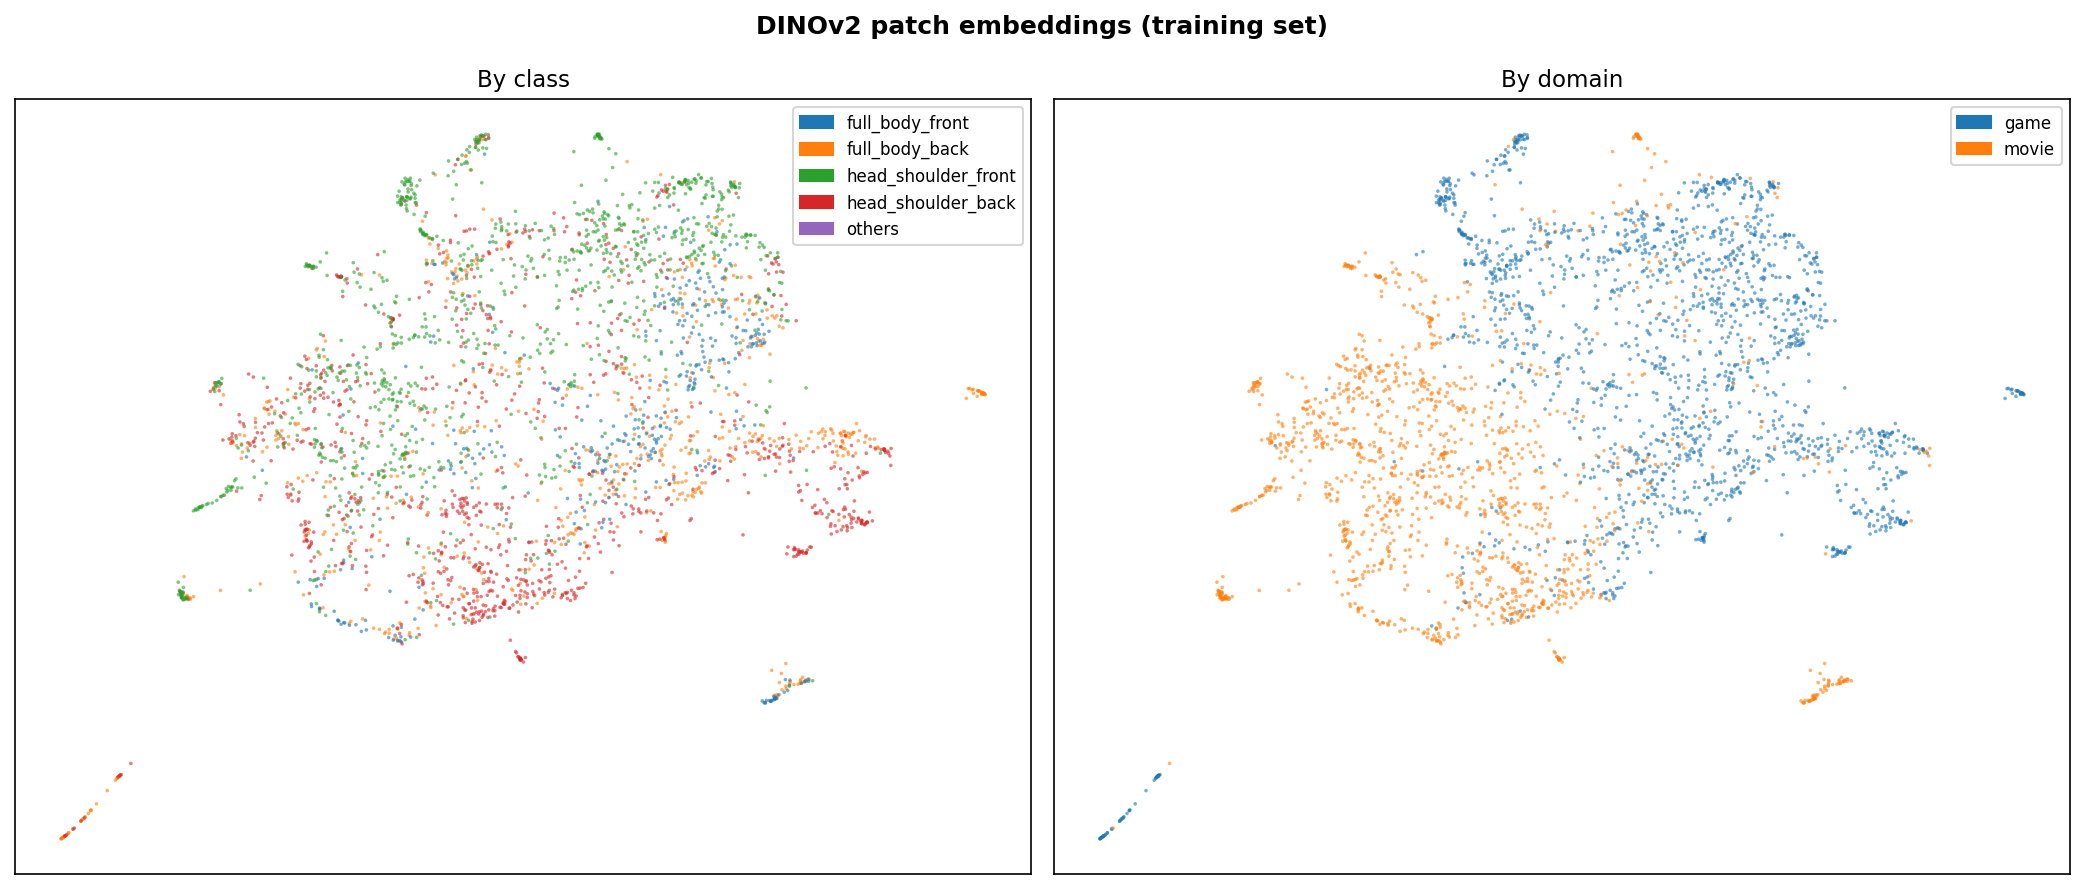
\includegraphics[width=\linewidth]{figs/dino_umap.png}
%   \caption{UMAP projection of DINOv2 embeddings for all training patches,
%            coloured by pose class (left) and domain (right). Clear clustering
%            motivates diversity-preserving selection.}
%   \label{fig:umap}
% \end{figure}


\section{Real-world Application}\label{s:rwa}

% ============================================================
% WORD LIMITS: 2.1 = 250w, 2.2 = 250w
% Excluded: equations, tables, figures, bibliography
% ============================================================

% ============================================================
\subsection{Image Model Deployment}
% ============================================================
% TASK: unpaired image-to-image translation on full frames (not patches).
%       Evaluate in both directions with metrics.
%       ≥10 success + ≥10 failure comparisons. 250 words.
%
% SUGGESTED STRUCTURE:
%
%   [Model] ~50 words
%     "We adopt Contrastive Unpaired Translation (CUT)~\cite{park2020},
%      which trains a generator \(G: A \to B\) using a PatchNCE loss
%      that maximises mutual information between input and output patches,
%      requiring no paired data.  We initialise from the publicly available
%      horse2zebra pretrained weights~\cite{park2020} and fine-tune for
%      5\,+\,3 epochs (constant LR then linear decay) on 500 full frames
%      per domain extracted at the timestamps of 1.1 detections
%      (GPU: NVIDIA Turing, $\sim$X minutes)."
%     Hardware: NVIDIA GeForce RTX 2080 Ti (NCC HPC cluster).
%     NOTE: fill in actual training time once you have it (check slurm logs).
%
%   [Evaluation] ~80 words
%     Metrics: FID (distribution-level quality), KID (unbiased FID),
%     LPIPS (perceptual patch similarity).
%     Report both directions: game→movie (AtoB) and movie→game (BtoA).
%     Example sentence:
%     "Table~\ref{tab:metrics21} reports FID, KID, and LPIPS in both
%      translation directions.  Game-to-movie translation achieves
%      FID\,=\,X / KID\,=\,X, reflecting the larger domain gap from
%      the constrained game palette to the varied cinematic style of
%      movie footage.  Movie-to-game (BtoA) is easier, yielding
%      FID\,=\,X, as the generator maps diverse movie textures to
%      the more homogeneous game rendering."
%
%   [Success cases] ~60 words
%     "Figure~\ref{fig:21_success} shows 10 successful translations.
%      The model consistently transfers film-grain texture and colour
%      grading to game frames, particularly for well-lit frontal shots
%      with clear clothing texture. [Add 1-2 specific visual observations
%      from your actual results, e.g., colour shift, grain, contrast.]"
%
%   [Failure cases] ~60 words
%     "Figure~\ref{fig:21_fail} shows 10 failure cases.
%      Common failures include: (1) background style leaking onto
%      foreground where YOLO bounding boxes were imprecise; (2) colour
%      artefacts on dark game scenes with low texture information;
%      (3) temporal inconsistency visible across consecutive frames
%      as the model has no inter-frame memory."
%
%   [Limitation] ~40 words
%     "The horse2zebra pretrained weights introduce a domain gap:
%      the generator's prior is tuned to animal textures rather than
%      human clothing.  Fine-tuning for only 8 epochs partially corrects
%      this; longer training or a more suitable pretrained base
%      (e.g.\ cityscapes) may improve results."
%
% KEY THINGS TO STATE:
%   - Hardware used and training time (explicitly required for marks)
%   - Both translation directions evaluated
%   - Why these metrics (FID = global distribution, LPIPS = local perceptual)
%   - Honest failure analysis (domain gap from horse2zebra, no temporal coherence)
%
% FIGURES:
%   Fig 4 — Metrics table.
%            Columns: Direction | FID ↓ | KID ↓ | LPIPS ↓
%            Rows: AtoB (game→movie), BtoA (movie→game)
%            Save to: paper/figs/ (as a LaTeX table, not image)
%
%   Fig 5 — Success cases: 2×5 or 5×2 grid, input|output pairs.
%            Pick 10 frames where the style transfer looks convincing.
%            From: output/q2_1/cut_data/testA/ (input)
%                  output/q2_1/<run>/fake_M/ (output)
%            Save to: paper/figs/success_21.pdf
%            Caption: "Successful game-to-movie translations (CUT, 2.1).
%                      Left: input game frame. Right: translated output."
%
%   Fig 6 — Failure cases: same format, 10 bad examples.
%            Save to: paper/figs/fail_21.pdf
%            Caption: "Failure cases: [describe 2-3 specific failure modes]."
%
% LATEX SKELETON:
% \begin{table}[t]
%   \centering
%   \caption{CUT translation metrics (2.1 full-frame model).
%            FID and KID measure distribution similarity; LPIPS measures
%            perceptual patch distance. Lower is better for all.}
%   \label{tab:metrics21}
%   \begin{tabular}{lrrr}
%     \toprule
%     Direction & FID\,↓ & KID\,↓ & LPIPS\,↓ \\
%     \midrule
%     Game $\to$ Movie (AtoB) & -- & -- & -- \\
%     Movie $\to$ Game (BtoA) & -- & -- & -- \\
%     \bottomrule
%   \end{tabular}
% \end{table}


% ============================================================
\subsection{Local (Temporal) Enhancement}
% ============================================================
% TASK: improve 2.1 using local (patch) methods and/or temporal approaches.
%       Submit enhanced video. ≥10 key-frame comparisons. 250 words.
%
% SUGGESTED STRUCTURE:
%
%   [Motivation] ~40 words
%     "The 2.1 model applies style transfer to full frames, mixing
%      foreground human style with background. We address this with
%      patch-level compositing: translating only detected human regions
%      and compositing them onto the original frame."
%
%   [Method overview] ~80 words
%     "For each test frame: (1) YOLO detects human bounding boxes;
%      (2) the 1.2 GCN classifies each patch, discarding `others';
%      (3) kept crops are translated by a CUT model fine-tuned on the
%      1.3-selected patches (game: X, movie: Y patches); (4) translated
%      crops are resized to original bbox dimensions and composited onto
%      the untranslated frame; (5) exponential moving average (EMA)
%      temporal blending (\(\alpha=0.3\)) reduces inter-frame flicker."
%     Fill in actual X, Y counts.
%
%   [Why patch fine-tuning helps] ~40 words
%     "Fine-tuning on human patches (vs.\ full frames) aligns the
%      generator's training distribution with the inference distribution:
%      the model sees the same crop scale and content at both train and
%      test time, reducing identity mapping artefacts."
%
%   [Evaluation — metrics] ~40 words
%     "Table~\ref{tab:metrics22} compares 2.1 and 2.2 metrics on the
%      same test splits.  The enhanced model achieves FID\,=\,X vs.\
%      2.1's Y, a Z\,\% improvement, confirming that patch-level
%      training narrows the domain gap for human regions."
%
%   [Key-frame comparison] ~30 words
%     "Figure~\ref{fig:keyframes} shows 10 key frames: original,
%      2.1 baseline, and 2.2 enhanced.  The patch compositing
%      preserves background fidelity while improving human-region
%      style consistency."
%
%   [Critical evaluation / failure analysis] ~60 words
%     "Remaining failure modes: (1) GCN misclassification of `others'
%      (9.8\% val accuracy) causes occasional style transfer on
%      non-human regions; (2) EMA blending introduces ghosting on fast
%      motion; (3) patch boundary artefacts are visible at bbox edges
%      due to hard compositing without feathering; (4) the horse2zebra
%      pretrained base still limits stylistic range."
%
% KEY THINGS TO STATE:
%   - Hardware: NVIDIA GeForce RTX 2080 Ti (NCC HPC cluster) — state this explicitly
%   - Training time for patch fine-tuning (check slurm logs for wall time)
%   - Explicit comparison to 2.1 (this is the main point)
%   - Both videos submitted (baseline 2.1 and enhanced 2.2)
%   - Honest failure analysis — the marker rewards critical thinking
%
% FIGURES:
%   Fig 7 — Metrics comparison table (2.1 vs 2.2).
%            Columns: Model | FID ↓ | KID ↓ | LPIPS ↓
%            Rows: 2.1 Full-frame CUT, 2.2 Patch CUT + EMA
%
%   Fig 8 — Key-frame comparison (≥10 frames required).
%            Three-column layout: Original | 2.1 Baseline | 2.2 Enhanced
%            Extract representative frames from:
%              output/q2_1/<run>/enhanced_video_21.mp4 (2.1)
%              output/q2_2/<run>/enhanced_model.mp4   (2.2)
%            Save individual frames as: paper/figs/kf_XX_orig.jpg etc.
%            or use a script to make a contact sheet.
%            Caption: "Key frame comparisons: original (left),
%                      2.1 full-frame CUT (centre), 2.2 patch-level
%                      CUT + EMA blending (right)."
%            Save to: paper/figs/keyframes_comparison.pdf
%
%   Fig 9 (optional but strong) — Patch compositing diagram.
%            Annotated figure showing:
%              (a) original frame with YOLO boxes drawn
%              (b) extracted patches
%              (c) translated patches
%              (d) composited result
%            Save to: paper/figs/compositing_pipeline.pdf
%            This is a diagram so word-count exempt and tells the story
%            of 2.2 at a glance.
%
% LATEX SKELETON:
% \begin{figure}[t]
%   \centering
%   \includegraphics[width=\linewidth]{figs/keyframes_comparison.pdf}
%   \caption{Ten key frames from the test video: original (left),
%            2.1 full-frame CUT baseline (centre), and 2.2 patch-level
%            CUT with EMA temporal blending (right).}
%   \label{fig:keyframes}
% \end{figure}
%
% \begin{table}[t]
%   \centering
%   \caption{Metric comparison between 2.1 and 2.2 models.}
%   \label{tab:metrics22}
%   \begin{tabular}{lrrr}
%     \toprule
%     Model & FID\,↓ & KID\,↓ & LPIPS\,↓ \\
%     \midrule
%     2.1 Full-frame CUT   & -- & -- & -- \\
%     2.2 Patch CUT + EMA  & -- & -- & -- \\
%     \bottomrule
%   \end{tabular}
% \end{table}


\section{Conclusion}


\bibliographystyle{plainnat}
\bibliography{ref}

\end{document}